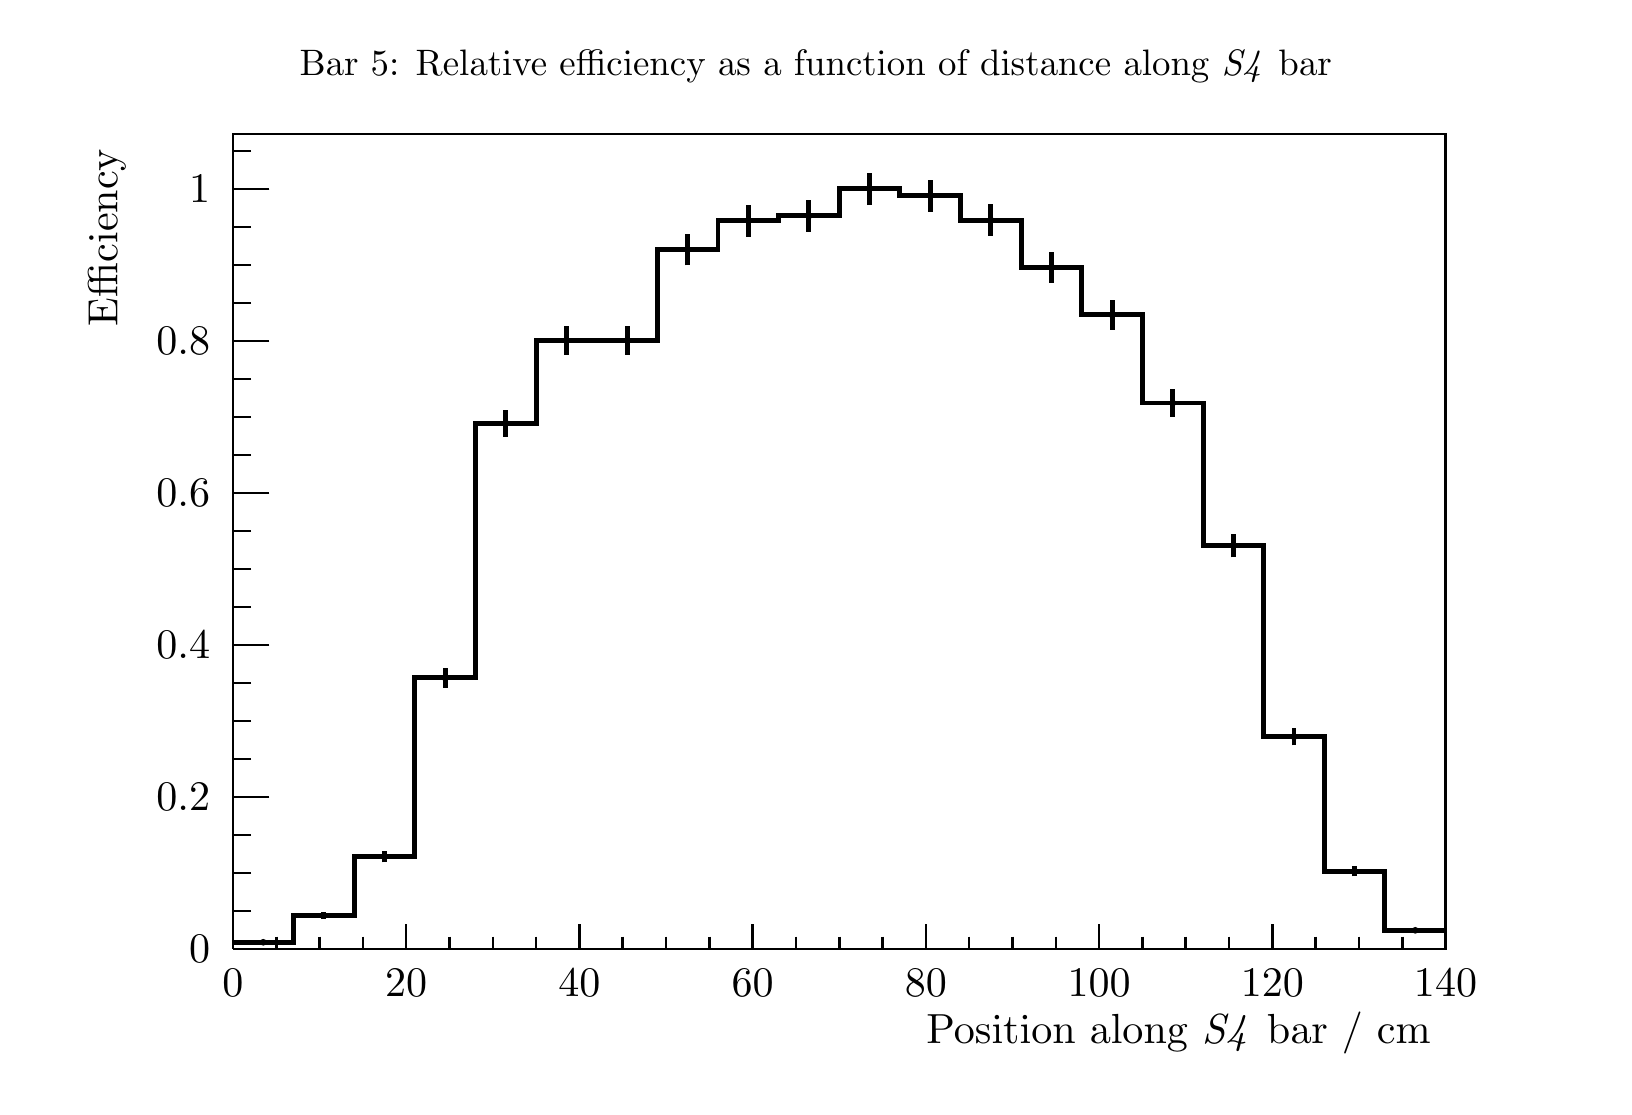
\begin{tikzpicture}
\pgfdeclareplotmark{cross} {
\pgfpathmoveto{\pgfpoint{-0.3\pgfplotmarksize}{\pgfplotmarksize}}
\pgfpathlineto{\pgfpoint{+0.3\pgfplotmarksize}{\pgfplotmarksize}}
\pgfpathlineto{\pgfpoint{+0.3\pgfplotmarksize}{0.3\pgfplotmarksize}}
\pgfpathlineto{\pgfpoint{+1\pgfplotmarksize}{0.3\pgfplotmarksize}}
\pgfpathlineto{\pgfpoint{+1\pgfplotmarksize}{-0.3\pgfplotmarksize}}
\pgfpathlineto{\pgfpoint{+0.3\pgfplotmarksize}{-0.3\pgfplotmarksize}}
\pgfpathlineto{\pgfpoint{+0.3\pgfplotmarksize}{-1.\pgfplotmarksize}}
\pgfpathlineto{\pgfpoint{-0.3\pgfplotmarksize}{-1.\pgfplotmarksize}}
\pgfpathlineto{\pgfpoint{-0.3\pgfplotmarksize}{-0.3\pgfplotmarksize}}
\pgfpathlineto{\pgfpoint{-1.\pgfplotmarksize}{-0.3\pgfplotmarksize}}
\pgfpathlineto{\pgfpoint{-1.\pgfplotmarksize}{0.3\pgfplotmarksize}}
\pgfpathlineto{\pgfpoint{-0.3\pgfplotmarksize}{0.3\pgfplotmarksize}}
\pgfpathclose
\pgfusepathqstroke
}
\pgfdeclareplotmark{cross*} {
\pgfpathmoveto{\pgfpoint{-0.3\pgfplotmarksize}{\pgfplotmarksize}}
\pgfpathlineto{\pgfpoint{+0.3\pgfplotmarksize}{\pgfplotmarksize}}
\pgfpathlineto{\pgfpoint{+0.3\pgfplotmarksize}{0.3\pgfplotmarksize}}
\pgfpathlineto{\pgfpoint{+1\pgfplotmarksize}{0.3\pgfplotmarksize}}
\pgfpathlineto{\pgfpoint{+1\pgfplotmarksize}{-0.3\pgfplotmarksize}}
\pgfpathlineto{\pgfpoint{+0.3\pgfplotmarksize}{-0.3\pgfplotmarksize}}
\pgfpathlineto{\pgfpoint{+0.3\pgfplotmarksize}{-1.\pgfplotmarksize}}
\pgfpathlineto{\pgfpoint{-0.3\pgfplotmarksize}{-1.\pgfplotmarksize}}
\pgfpathlineto{\pgfpoint{-0.3\pgfplotmarksize}{-0.3\pgfplotmarksize}}
\pgfpathlineto{\pgfpoint{-1.\pgfplotmarksize}{-0.3\pgfplotmarksize}}
\pgfpathlineto{\pgfpoint{-1.\pgfplotmarksize}{0.3\pgfplotmarksize}}
\pgfpathlineto{\pgfpoint{-0.3\pgfplotmarksize}{0.3\pgfplotmarksize}}
\pgfpathclose
\pgfusepathqfillstroke
}
\pgfdeclareplotmark{newstar} {
\pgfpathmoveto{\pgfqpoint{0pt}{\pgfplotmarksize}}
\pgfpathlineto{\pgfqpointpolar{44}{0.5\pgfplotmarksize}}
\pgfpathlineto{\pgfqpointpolar{18}{\pgfplotmarksize}}
\pgfpathlineto{\pgfqpointpolar{-20}{0.5\pgfplotmarksize}}
\pgfpathlineto{\pgfqpointpolar{-54}{\pgfplotmarksize}}
\pgfpathlineto{\pgfqpointpolar{-90}{0.5\pgfplotmarksize}}
\pgfpathlineto{\pgfqpointpolar{234}{\pgfplotmarksize}}
\pgfpathlineto{\pgfqpointpolar{198}{0.5\pgfplotmarksize}}
\pgfpathlineto{\pgfqpointpolar{162}{\pgfplotmarksize}}
\pgfpathlineto{\pgfqpointpolar{134}{0.5\pgfplotmarksize}}
\pgfpathclose
\pgfusepathqstroke
}
\pgfdeclareplotmark{newstar*} {
\pgfpathmoveto{\pgfqpoint{0pt}{\pgfplotmarksize}}
\pgfpathlineto{\pgfqpointpolar{44}{0.5\pgfplotmarksize}}
\pgfpathlineto{\pgfqpointpolar{18}{\pgfplotmarksize}}
\pgfpathlineto{\pgfqpointpolar{-20}{0.5\pgfplotmarksize}}
\pgfpathlineto{\pgfqpointpolar{-54}{\pgfplotmarksize}}
\pgfpathlineto{\pgfqpointpolar{-90}{0.5\pgfplotmarksize}}
\pgfpathlineto{\pgfqpointpolar{234}{\pgfplotmarksize}}
\pgfpathlineto{\pgfqpointpolar{198}{0.5\pgfplotmarksize}}
\pgfpathlineto{\pgfqpointpolar{162}{\pgfplotmarksize}}
\pgfpathlineto{\pgfqpointpolar{134}{0.5\pgfplotmarksize}}
\pgfpathclose
\pgfusepathqfillstroke
}
\definecolor{c}{rgb}{1,1,1};
\draw [color=c, fill=c] (0,0) rectangle (20,13.4379);
\draw [color=c, fill=c] (2.6,1.74693) rectangle (18,12.0942);
\definecolor{c}{rgb}{0,0,0};
\draw [c,line width=0.9] (2.6,1.74693) -- (2.6,12.0942) -- (18,12.0942) -- (18,1.74693) -- (2.6,1.74693);
\definecolor{c}{rgb}{1,1,1};
\draw [color=c, fill=c] (2.6,1.74693) rectangle (18,12.0942);
\definecolor{c}{rgb}{0,0,0};
\draw [c,line width=0.9] (2.6,1.74693) -- (2.6,12.0942) -- (18,12.0942) -- (18,1.74693) -- (2.6,1.74693);
\draw [c,line width=1.8] (2.985,1.81052) -- (2.985,1.82945);
\draw [c,line width=1.8] (2.985,1.82945) -- (2.985,1.84838);
\foreach \P in {(2.985,1.82945)}{\draw[mark options={color=c,fill=c},mark size=2.402402pt,mark=*,mark size=1pt] plot coordinates {\P};}
\draw [c,line width=1.8] (3.755,2.12542) -- (3.755,2.16819);
\draw [c,line width=1.8] (3.755,2.16819) -- (3.755,2.21096);
\foreach \P in {(3.755,2.16819)}{\draw[mark options={color=c,fill=c},mark size=2.402402pt,mark=*,mark size=1pt] plot coordinates {\P};}
\draw [c,line width=1.8] (4.525,2.84393) -- (4.525,2.91516);
\draw [c,line width=1.8] (4.525,2.91516) -- (4.525,2.98638);
\foreach \P in {(4.525,2.91516)}{\draw[mark options={color=c,fill=c},mark size=2.402402pt,mark=*,mark size=1pt] plot coordinates {\P};}
\draw [c,line width=1.8] (5.295,5.06424) -- (5.295,5.18646);
\draw [c,line width=1.8] (5.295,5.18646) -- (5.295,5.30868);
\foreach \P in {(5.295,5.18646)}{\draw[mark options={color=c,fill=c},mark size=2.402402pt,mark=*,mark size=1pt] plot coordinates {\P};}
\draw [c,line width=1.8] (6.065,8.25161) -- (6.065,8.42187);
\draw [c,line width=1.8] (6.065,8.42187) -- (6.065,8.59213);
\foreach \P in {(6.065,8.42187)}{\draw[mark options={color=c,fill=c},mark size=2.402402pt,mark=*,mark size=1pt] plot coordinates {\P};}
\draw [c,line width=1.8] (6.835,9.29396) -- (6.835,9.47718);
\draw [c,line width=1.8] (6.835,9.47718) -- (6.835,9.6604);
\foreach \P in {(6.835,9.47718)}{\draw[mark options={color=c,fill=c},mark size=2.402402pt,mark=*,mark size=1pt] plot coordinates {\P};}
\draw [c,line width=1.8] (7.605,9.28966) -- (7.605,9.47284);
\draw [c,line width=1.8] (7.605,9.47284) -- (7.605,9.65601);
\foreach \P in {(7.605,9.47284)}{\draw[mark options={color=c,fill=c},mark size=2.402402pt,mark=*,mark size=1pt] plot coordinates {\P};}
\draw [c,line width=1.8] (8.375,10.4273) -- (8.375,10.6237);
\draw [c,line width=1.8] (8.375,10.6237) -- (8.375,10.82);
\foreach \P in {(8.375,10.6237)}{\draw[mark options={color=c,fill=c},mark size=2.402402pt,mark=*,mark size=1pt] plot coordinates {\P};}
\draw [c,line width=1.8] (9.145,10.7924) -- (9.145,10.9928);
\draw [c,line width=1.8] (9.145,10.9928) -- (9.145,11.1932);
\foreach \P in {(9.145,10.9928)}{\draw[mark options={color=c,fill=c},mark size=2.402402pt,mark=*,mark size=1pt] plot coordinates {\P};}
\draw [c,line width=1.8] (9.915,10.8526) -- (9.915,11.0536);
\draw [c,line width=1.8] (9.915,11.0536) -- (9.915,11.2547);
\foreach \P in {(9.915,11.0536)}{\draw[mark options={color=c,fill=c},mark size=2.402402pt,mark=*,mark size=1pt] plot coordinates {\P};}
\draw [c,line width=1.8] (10.685,11.192) -- (10.685,11.3967);
\draw [c,line width=1.8] (10.685,11.3967) -- (10.685,11.6014);
\foreach \P in {(10.685,11.3967)}{\draw[mark options={color=c,fill=c},mark size=2.402402pt,mark=*,mark size=1pt] plot coordinates {\P};}
\draw [c,line width=1.8] (11.455,11.1061) -- (11.455,11.3099);
\draw [c,line width=1.8] (11.455,11.3099) -- (11.455,11.5136);
\foreach \P in {(11.455,11.3099)}{\draw[mark options={color=c,fill=c},mark size=2.402402pt,mark=*,mark size=1pt] plot coordinates {\P};}
\draw [c,line width=1.8] (12.225,10.801) -- (12.225,11.0015);
\draw [c,line width=1.8] (12.225,11.0015) -- (12.225,11.202);
\foreach \P in {(12.225,11.0015)}{\draw[mark options={color=c,fill=c},mark size=2.402402pt,mark=*,mark size=1pt] plot coordinates {\P};}
\draw [c,line width=1.8] (12.995,10.204) -- (12.995,10.3979);
\draw [c,line width=1.8] (12.995,10.3979) -- (12.995,10.5917);
\foreach \P in {(12.995,10.3979)}{\draw[mark options={color=c,fill=c},mark size=2.402402pt,mark=*,mark size=1pt] plot coordinates {\P};}
\draw [c,line width=1.8] (13.765,9.61156) -- (13.765,9.79855);
\draw [c,line width=1.8] (13.765,9.79855) -- (13.765,9.98554);
\foreach \P in {(13.765,9.79855)}{\draw[mark options={color=c,fill=c},mark size=2.402402pt,mark=*,mark size=1pt] plot coordinates {\P};}
\draw [c,line width=1.8] (14.535,8.5046) -- (14.535,8.6781);
\draw [c,line width=1.8] (14.535,8.6781) -- (14.535,8.85159);
\foreach \P in {(14.535,8.6781)}{\draw[mark options={color=c,fill=c},mark size=2.402402pt,mark=*,mark size=1pt] plot coordinates {\P};}
\draw [c,line width=1.8] (15.305,6.71802) -- (15.305,6.86714);
\draw [c,line width=1.8] (15.305,6.86714) -- (15.305,7.01625);
\foreach \P in {(15.305,6.86714)}{\draw[mark options={color=c,fill=c},mark size=2.402402pt,mark=*,mark size=1pt] plot coordinates {\P};}
\draw [c,line width=1.8] (16.075,4.33136) -- (16.075,4.43949);
\draw [c,line width=1.8] (16.075,4.43949) -- (16.075,4.54763);
\foreach \P in {(16.075,4.43949)}{\draw[mark options={color=c,fill=c},mark size=2.402402pt,mark=*,mark size=1pt] plot coordinates {\P};}
\draw [c,line width=1.8] (16.845,2.66733) -- (16.845,2.73276);
\draw [c,line width=1.8] (16.845,2.73276) -- (16.845,2.79819);
\foreach \P in {(16.845,2.73276)}{\draw[mark options={color=c,fill=c},mark size=2.402402pt,mark=*,mark size=1pt] plot coordinates {\P};}
\draw [c,line width=1.8] (17.615,1.94953) -- (17.615,1.98145);
\draw [c,line width=1.8] (17.615,1.98145) -- (17.615,2.01336);
\foreach \P in {(17.615,1.98145)}{\draw[mark options={color=c,fill=c},mark size=2.402402pt,mark=*,mark size=1pt] plot coordinates {\P};}
\draw [c,line width=1.8] (2.6,1.82945) -- (3.37,1.82945) -- (3.37,2.16819) -- (4.14,2.16819) -- (4.14,2.91516) -- (4.91,2.91516) -- (4.91,5.18646) -- (5.68,5.18646) -- (5.68,8.42187) -- (6.45,8.42187) -- (6.45,9.47718) -- (7.22,9.47718) --
 (7.22,9.47284) -- (7.99,9.47284) -- (7.99,10.6237) -- (8.76,10.6237) -- (8.76,10.9928) -- (9.53,10.9928) -- (9.53,11.0536) -- (10.3,11.0536) -- (10.3,11.3967) -- (11.07,11.3967) -- (11.07,11.3099) -- (11.84,11.3099) -- (11.84,11.0015) --
 (12.61,11.0015) -- (12.61,10.3979) -- (13.38,10.3979) -- (13.38,9.79855) -- (14.15,9.79855) -- (14.15,8.6781) -- (14.92,8.6781) -- (14.92,6.86714) -- (15.69,6.86714) -- (15.69,4.43949) -- (16.46,4.43949) -- (16.46,2.73276) -- (17.23,2.73276) --
 (17.23,1.98145) -- (18,1.98145);
\draw [c,line width=0.9] (2.6,1.74693) -- (18,1.74693);
\draw [c,line width=0.9] (2.6,2.05735) -- (2.6,1.74693);
\draw [c,line width=0.9] (3.15,1.90214) -- (3.15,1.74693);
\draw [c,line width=0.9] (3.7,1.90214) -- (3.7,1.74693);
\draw [c,line width=0.9] (4.25,1.90214) -- (4.25,1.74693);
\draw [c,line width=0.9] (4.8,2.05735) -- (4.8,1.74693);
\draw [c,line width=0.9] (5.35,1.90214) -- (5.35,1.74693);
\draw [c,line width=0.9] (5.9,1.90214) -- (5.9,1.74693);
\draw [c,line width=0.9] (6.45,1.90214) -- (6.45,1.74693);
\draw [c,line width=0.9] (7,2.05735) -- (7,1.74693);
\draw [c,line width=0.9] (7.55,1.90214) -- (7.55,1.74693);
\draw [c,line width=0.9] (8.1,1.90214) -- (8.1,1.74693);
\draw [c,line width=0.9] (8.65,1.90214) -- (8.65,1.74693);
\draw [c,line width=0.9] (9.2,2.05735) -- (9.2,1.74693);
\draw [c,line width=0.9] (9.75,1.90214) -- (9.75,1.74693);
\draw [c,line width=0.9] (10.3,1.90214) -- (10.3,1.74693);
\draw [c,line width=0.9] (10.85,1.90214) -- (10.85,1.74693);
\draw [c,line width=0.9] (11.4,2.05735) -- (11.4,1.74693);
\draw [c,line width=0.9] (11.95,1.90214) -- (11.95,1.74693);
\draw [c,line width=0.9] (12.5,1.90214) -- (12.5,1.74693);
\draw [c,line width=0.9] (13.05,1.90214) -- (13.05,1.74693);
\draw [c,line width=0.9] (13.6,2.05735) -- (13.6,1.74693);
\draw [c,line width=0.9] (14.15,1.90214) -- (14.15,1.74693);
\draw [c,line width=0.9] (14.7,1.90214) -- (14.7,1.74693);
\draw [c,line width=0.9] (15.25,1.90214) -- (15.25,1.74693);
\draw [c,line width=0.9] (15.8,2.05735) -- (15.8,1.74693);
\draw [c,line width=0.9] (16.35,1.90214) -- (16.35,1.74693);
\draw [c,line width=0.9] (16.9,1.90214) -- (16.9,1.74693);
\draw [c,line width=0.9] (17.45,1.90214) -- (17.45,1.74693);
\draw [c,line width=0.9] (18,2.05735) -- (18,1.74693);
\draw [anchor=base] (2.6,1.14223) node[scale=1.52078, color=c, rotate=0]{0};
\draw [anchor=base] (4.8,1.14223) node[scale=1.52078, color=c, rotate=0]{20};
\draw [anchor=base] (7,1.14223) node[scale=1.52078, color=c, rotate=0]{40};
\draw [anchor=base] (9.2,1.14223) node[scale=1.52078, color=c, rotate=0]{60};
\draw [anchor=base] (11.4,1.14223) node[scale=1.52078, color=c, rotate=0]{80};
\draw [anchor=base] (13.6,1.14223) node[scale=1.52078, color=c, rotate=0]{100};
\draw [anchor=base] (15.8,1.14223) node[scale=1.52078, color=c, rotate=0]{120};
\draw [anchor=base] (18,1.14223) node[scale=1.52078, color=c, rotate=0]{140};
\draw [anchor= east] (18,0.671897) node[scale=1.52078, color=c, rotate=0]{Position along $\mathit{S4}$ bar / cm};
\draw [c,line width=0.9] (2.6,1.74693) -- (2.6,12.0942);
\draw [c,line width=0.9] (3.062,1.74693) -- (2.6,1.74693);
\draw [c,line width=0.9] (2.831,2.22942) -- (2.6,2.22942);
\draw [c,line width=0.9] (2.831,2.71191) -- (2.6,2.71191);
\draw [c,line width=0.9] (2.831,3.1944) -- (2.6,3.1944);
\draw [c,line width=0.9] (3.062,3.67689) -- (2.6,3.67689);
\draw [c,line width=0.9] (2.831,4.15938) -- (2.6,4.15938);
\draw [c,line width=0.9] (2.831,4.64187) -- (2.6,4.64187);
\draw [c,line width=0.9] (2.831,5.12436) -- (2.6,5.12436);
\draw [c,line width=0.9] (3.062,5.60684) -- (2.6,5.60684);
\draw [c,line width=0.9] (2.831,6.08933) -- (2.6,6.08933);
\draw [c,line width=0.9] (2.831,6.57182) -- (2.6,6.57182);
\draw [c,line width=0.9] (2.831,7.05431) -- (2.6,7.05431);
\draw [c,line width=0.9] (3.062,7.5368) -- (2.6,7.5368);
\draw [c,line width=0.9] (2.831,8.01929) -- (2.6,8.01929);
\draw [c,line width=0.9] (2.831,8.50178) -- (2.6,8.50178);
\draw [c,line width=0.9] (2.831,8.98427) -- (2.6,8.98427);
\draw [c,line width=0.9] (3.062,9.46676) -- (2.6,9.46676);
\draw [c,line width=0.9] (2.831,9.94925) -- (2.6,9.94925);
\draw [c,line width=0.9] (2.831,10.4317) -- (2.6,10.4317);
\draw [c,line width=0.9] (2.831,10.9142) -- (2.6,10.9142);
\draw [c,line width=0.9] (3.062,11.3967) -- (2.6,11.3967);
\draw [c,line width=0.9] (3.062,11.3967) -- (2.6,11.3967);
\draw [c,line width=0.9] (2.831,11.8792) -- (2.6,11.8792);
\draw [anchor= east] (2.5,1.74693) node[scale=1.52078, color=c, rotate=0]{0};
\draw [anchor= east] (2.5,3.67689) node[scale=1.52078, color=c, rotate=0]{0.2};
\draw [anchor= east] (2.5,5.60684) node[scale=1.52078, color=c, rotate=0]{0.4};
\draw [anchor= east] (2.5,7.5368) node[scale=1.52078, color=c, rotate=0]{0.6};
\draw [anchor= east] (2.5,9.46676) node[scale=1.52078, color=c, rotate=0]{0.8};
\draw [anchor= east] (2.5,11.3967) node[scale=1.52078, color=c, rotate=0]{1};
\draw [anchor= east] (1,12.0942) node[scale=1.52078, color=c, rotate=90]{Efficiency};
\draw (10,12.9599) node[scale=1.33068, color=c, rotate=0]{Bar 5: Relative efficiency as a function of distance along $\mathit{S4}$ bar};
\end{tikzpicture}
